\chapter{Work Plan}

To accomplish the objective of this doctoral research, we compose the work plan for our time line that generally consists of:

\begin{enumerate}

\item Data acquisition and data processing of several radio galaxies from ALMA calibrator public data

\item Developing the automation script to analyze new incoming ALMA's calibrator data 

\item Analyzing the data to derive some basic parameters of radio galaxy in (sub)mm region and improving the dynamic range of 
the corresponding image

\item Analyzing the data and the environment of radio galaxies incorporating the observational data from other wavelenghts

\end{enumerate} 

We note that some works in developing the automation scripts have been completed and they were used to process about 10 sources. More sources are certainly in progress. Since this work is in a cooperation framework with the JAO, some parts of the jobs is previewed to be conducted in ALMA Santiago Center Office (SCO), Chile. A short visit in 2017 (4 months), from April to July, has allowed to complete the basic tools necessary for the job. Next visit in the scheme of ESO Studentship is planned from April 2018 to April 2019. 

In dealing with huge data such as ALMA science projects, we certainly needs good infrastructures, namely a reliable internet connection, computer clusters, sufficient disk space, and reliable laptops. Fortunately, this facility can be provided more or less adequately. When we stay in Santiago, we use the ALMA Cluster (almascoop) which is avalable almost permanently. In ITB, we use Perseus Cluster (running with 16 processor) and another Workstation (running with 8 processors). An ordinary Linux desktop (with i3 processor) is also avalable to share the job. In total, we have approximately 15 Tb of space disk available to conduct this work, albeit some space must be shared with others. We are also granted from the ITB Network Administration an unlimited quota of internet connection to conduct this work.  

It remains to find an effective and efficient way to manage the transfer of these huge data between different machines in order to allow saving time. The timeline describing those steps are shown in \autoref{fig:workplan}.


\begin{landscape}
\begin{figure}[!ht]
\centering
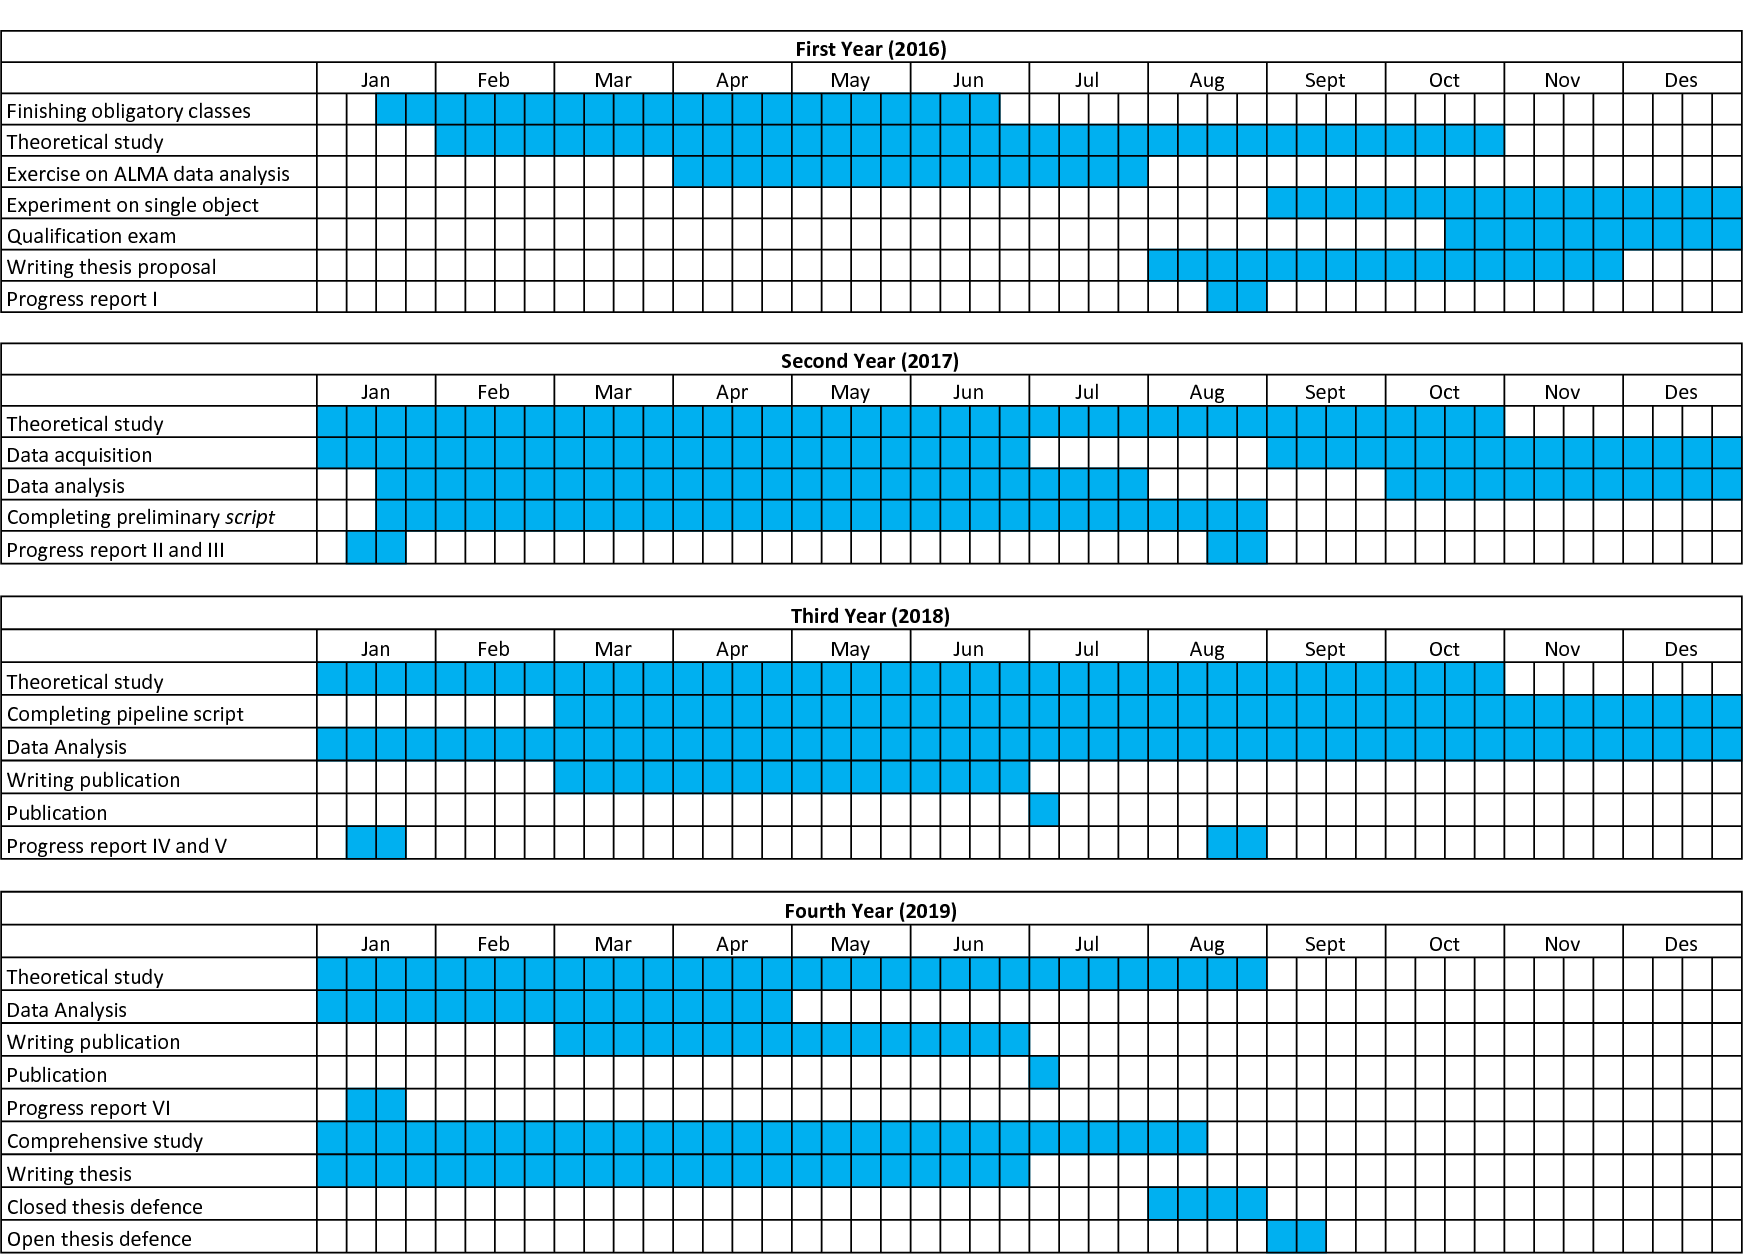
\includegraphics[scale=0.3]{fig/workplan.png}
\caption{Work plan for the first, second, third, and fourth year of doctoral study.}
\label{fig:workplan}
\end{figure}
\end{landscape}

\cleardoublepage
